\documentclass[a4paper, 11pt]{article}
%
\usepackage[utf8]{inputenc}
\usepackage[T1]{fontenc}
\usepackage{lmodern}
\usepackage[francais]{babel}
\usepackage[top=1cm, bottom=1cm, left=1cm, right=2cm]{geometry}
\usepackage{nopageno}
\usepackage{graphicx}
%
\newcommand{\env}[1]{\fbox{\begin{minipage}{\textwidth}#1\end{minipage}}}
%
\title{Exo SD 3 Arbres}
\author{Sarfraz \bsc{kapasi}}
\date{02/11/2012}
%
\begin{document}
%
\maketitle
%
\section{Conversion d'arbres en listes}
Voici quelques schémas représentant des arbres (représentation externe) ; représentez-les sous forme de liste :
\begin{enumerate}
  \item \frame{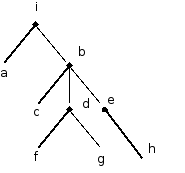
\includegraphics[height=120pt, width=180pt]{Arbre1.png}}
Réponse: (i (a) (b (c) (d (f) (g)) (e (h))))
  \item \frame{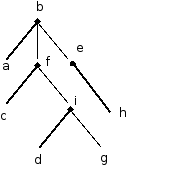
\includegraphics[height=120pt, width=180pt]{Arbre2.png}}
Réponse: (b (a) (f (c) (i (d) (g))) (e (h)))
  \item \frame{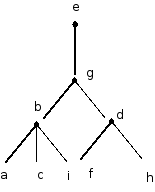
\includegraphics[height=120pt, width=180pt]{Arbre3.png}}
Réponse: (e (g (b (a) (c) (i)) (d (f) (h))))
  \item \frame{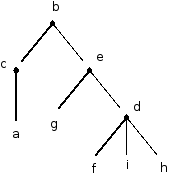
\includegraphics[height=120pt, width=180pt]{Arbre4.png}}
Réponse: (b (c (a)) (e (g) (d (f) (i) (h))))
  \item \frame{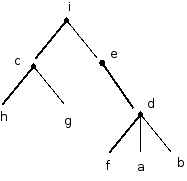
\includegraphics[height=120pt, width=180pt]{Arbre5.png}}
Réponse: (i (c (h) (g)) (e (d (f) (a) (b))))
  \item \frame{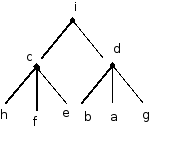
\includegraphics[height=120pt, width=180pt]{Arbre6.png}}
Réponse: (i (c (h) (f) (e)) (d (b) (a) (g)))
\end{enumerate}

\section{Conversion de listes en arbres}
Voici quelques représentations internes d'arbres sous forme de listes ; à l'aide de Dia, en utilisant la feuille Arbre, tracez leur représentation externe (sous forme de schéma) :
\begin{enumerate}
    \item (a (b (c (d) (e) (f))) (g (h) (i)))\\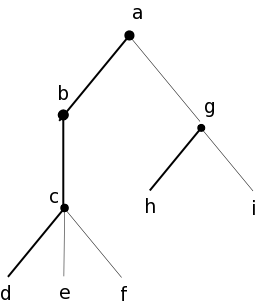
\includegraphics[scale=0.3]{reponse1.png}
    \item (b (i (d) (e) (f (g (h)) (c))) (a))\\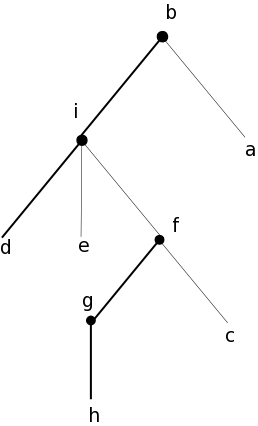
\includegraphics[scale=0.3]{reponse2.png}
    \item (a (i (c (b (e (h))) (g (d)) (f))))\\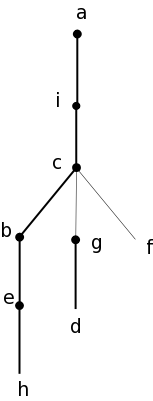
\includegraphics[scale=0.3]{reponse3.png}
    \item (a (d (e (b (c (f))) (g)) (i)) (h))\\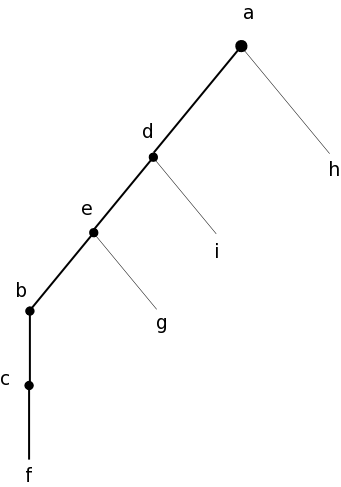
\includegraphics[scale=0.3]{reponse4.png}
    \item (i (b (e (h)) (a)) (f) (c) (d (g)))\\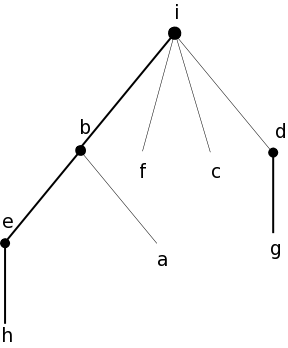
\includegraphics[scale=0.3]{reponse5.png}
    \item (h (f (g (b)) (i (d) (e)) (c (a))))\\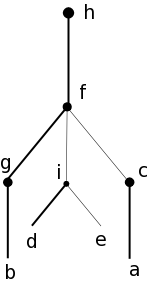
\includegraphics[scale=0.3]{reponse6.png}
\end{enumerate}

\end{document}
